\documentclass[tikz,border=10pt]{standalone}
\usepackage{amsmath}
\usepackage{amssymb}
\usepackage{tikz}
\usetikzlibrary{arrows.meta,calc}

\definecolor{figazul}{RGB}{2,132,199}
\definecolor{figrojo}{RGB}{220,38,38}
\definecolor{figverde}{RGB}{22,163,74}

\begin{document}
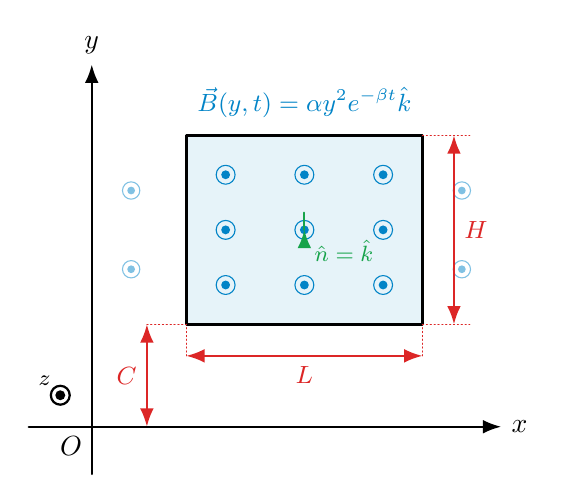
\begin{tikzpicture}[>=Latex, line cap=round, line join=round]
  % Ejes coordenados x, y
  \draw[->, thick] (-0.8, 0) -- (5.2, 0) node[right] {$x$};
  \draw[->, thick] (0, -0.6) -- (0, 4.6) node[above] {$y$};
  \node[below left] at (0,0) {$O$};

  % Eje z saliente cerca del origen
  \draw[thick] (-0.4, 0.4) circle (0.12);
  \fill (-0.4, 0.4) circle (1.8pt);
  \node[above left, font=\footnotesize] at (-0.4, 0.4) {$z$};

  % Rectángulo conductor de lados L x H
  % Ubicado en x de 1.2 a 4.2 (L = 3.0)
  % y de C = 1.3 a C+H = 3.7 (H = 2.4)
  \draw[very thick, fill=figazul!10] (1.2, 1.3) rectangle (4.2, 3.7);

  % Grilla regular de campo magnético saliente B(y,t) (\odot)
  \foreach \gx in {1.7, 2.7, 3.7} {
    \foreach \gy in {1.8, 2.5, 3.2} {
      \draw[thin, color=figazul] (\gx, \gy) circle (0.12);
      \fill[color=figazul] (\gx, \gy) circle (1.6pt);
    }
  }
  % Puntos adicionales de campo fuera para indicar campo en la región
  \foreach \gx in {0.5, 4.7} {
    \foreach \gy in {2.0, 3.0} {
      \draw[thin, color=figazul!50] (\gx, \gy) circle (0.11);
      \fill[color=figazul!50] (\gx, \gy) circle (1.4pt);
    }
  }
  \node[above, font=\small, color=figazul] at (2.7, 3.8) {$\vec{B}(y,t) = \alpha y^2 e^{-\beta t}\hat{k}$};

  % Cotas en rojo
  % Cota C desde el eje x hasta el lado inferior
  \draw[<->, thick, color=figrojo] (0.7, 0) -- (0.7, 1.3) node[midway, left, color=figrojo, font=\small] {$C$};
  \draw[densely dotted, thin, color=figrojo] (0.7, 1.3) -- (1.2, 1.3);

  % Cota H para la altura del rectángulo
  \draw[<->, thick, color=figrojo] (4.6, 1.3) -- (4.6, 3.7) node[midway, right, color=figrojo, font=\small] {$H$};
  \draw[densely dotted, thin, color=figrojo] (4.2, 1.3) -- (4.8, 1.3);
  \draw[densely dotted, thin, color=figrojo] (4.2, 3.7) -- (4.8, 3.7);

  % Cota L para el ancho del rectángulo
  \draw[<->, thick, color=figrojo] (1.2, 0.9) -- (4.2, 0.9) node[midway, below, color=figrojo, font=\small] {$L$};
  \draw[densely dotted, thin, color=figrojo] (1.2, 0.9) -- (1.2, 1.3);
  \draw[densely dotted, thin, color=figrojo] (4.2, 0.9) -- (4.2, 1.3);

  % Vector normal n_hat = k_hat
  \draw[->, thick, color=figverde] (2.7, 2.5) -- (2.7, 2.5) node[below right, color=figverde, font=\footnotesize] {$\hat{n} = \hat{k}$};

\end{tikzpicture}
\end{document}
